
    \begin{picture} (220.000000,263.600000)(0,0)
    \put(0.0, 0.0){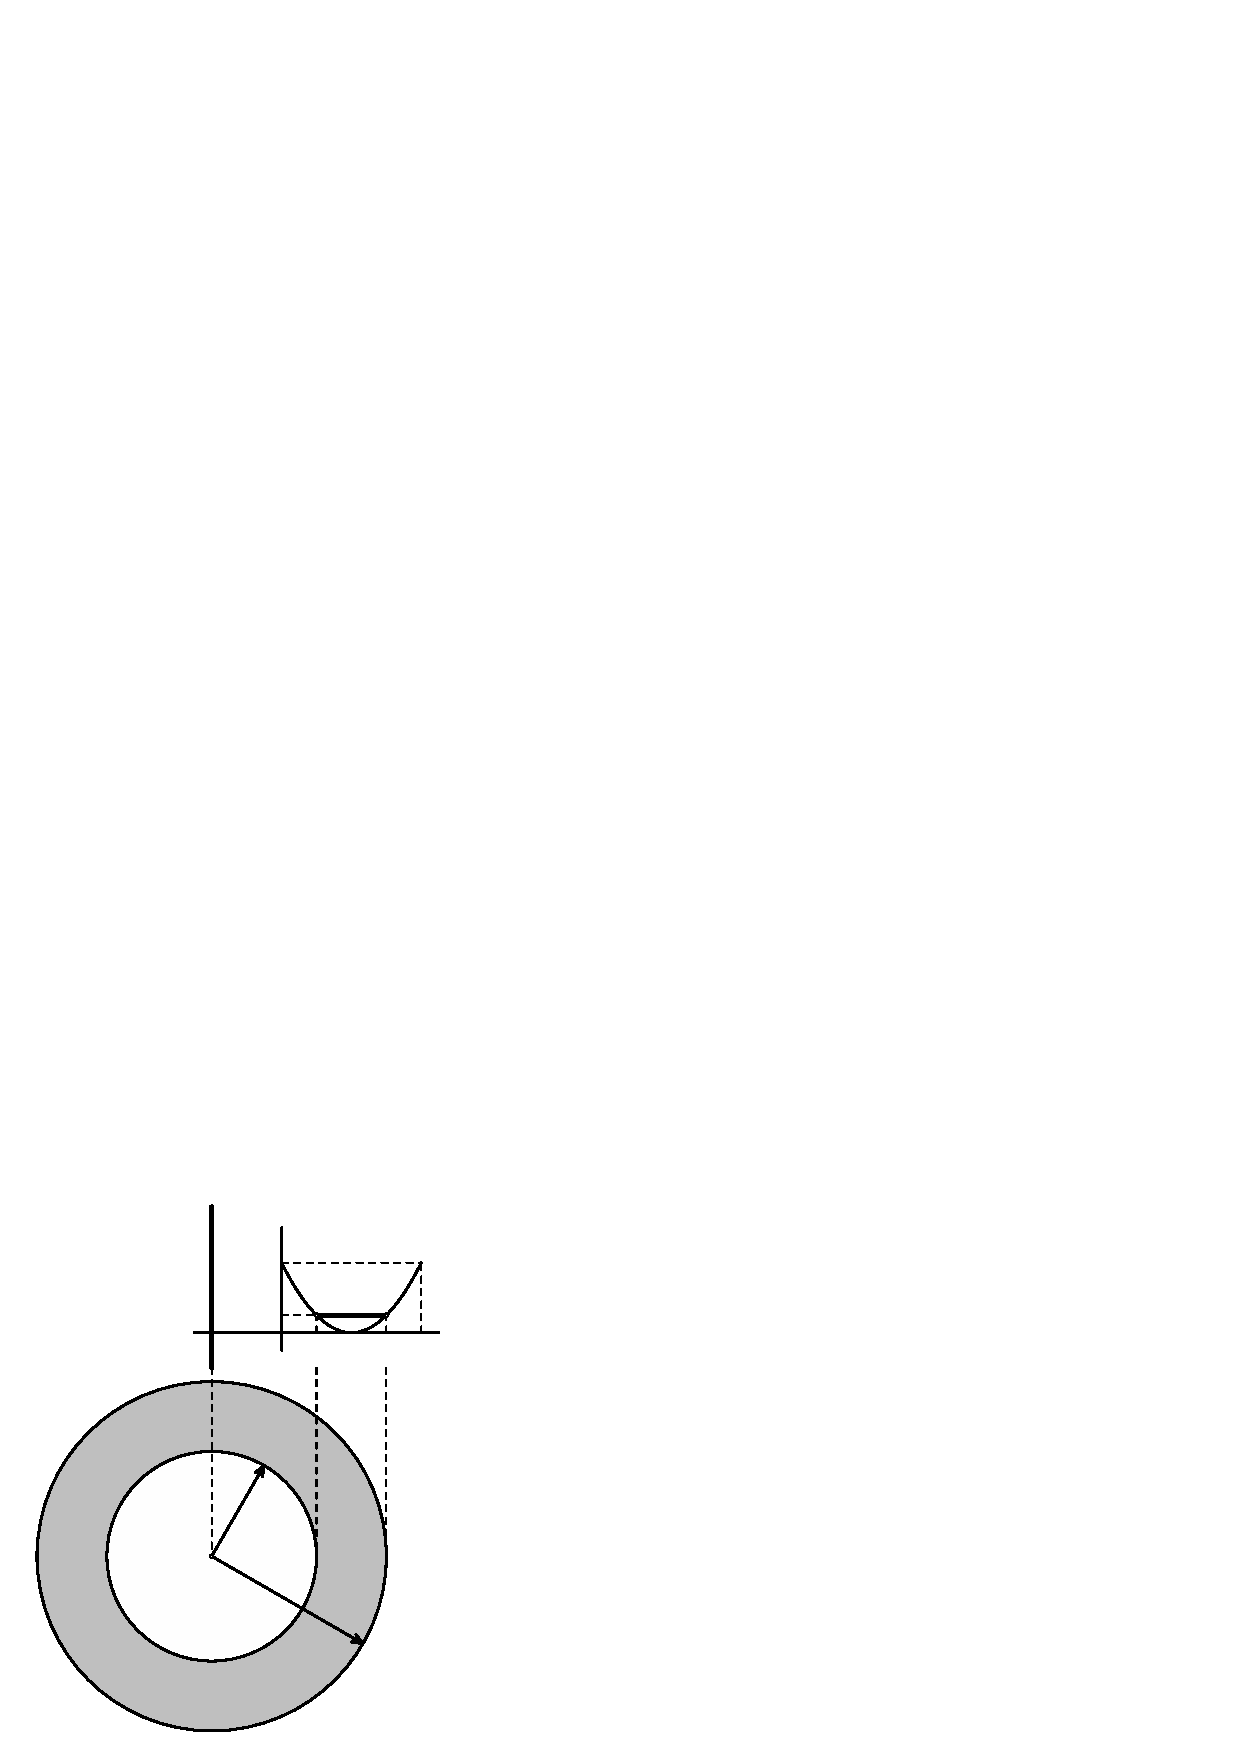
\includegraphics{09bowl_variation1.pdf}}
        \put(190.23, 239.77){\sffamily\itshape $y=(x-1)^2$}
    \put(151.92, 214.62){\sffamily\itshape $A$}
    \put(181.46, 214.62){\sffamily\itshape $B$}
    \put(149.92, 192.23){\sffamily\itshape $x_{\mathrm{in}}$}
    \put(116.19, 110.69){\sffamily\itshape $r_{\mathrm{in}}$}
    \put(183.46, 192.23){\sffamily\itshape $x_{\mathrm{out}}$}
    \put(152.66,  70.06){\sffamily\itshape $r_{\mathrm{out}}$}
    \put(212.29, 202.23){\sffamily\itshape $x$}
    \put(128.15, 234.77){\sffamily\itshape 1}
    \put(166.69, 192.23){\sffamily\itshape 1}
    \put(200.23, 192.23){\sffamily\itshape 2}
    \put(128.15, 209.62){\sffamily\itshape $y$}
    \put(101.62,  28.07){\sffamily\itshape \makebox[0pt][c]{Area$=\pi r_{\rm out}^2-\pi r_{\rm in}^2$}}
    \put( 92.62, 205.23){\sffamily\itshape \rotatebox{90}{Rotation axis}}
    \put( 34.54, 235.77){\sffamily\itshape SIDE VIEW:}
    \put( 34.54, 185.46){\sffamily\itshape TOP VIEW:}
\end{picture}
